\chapter{Requirements and Specification}

After a short introduction to the basic terms and Apache Flink and Apache Kafka in
context of big data and stream processing, this chapter describes Data Quality and
presents common criteria to measure the quality of data. Based on this criteria, available data
for both of the systems will be inspected to build the foundation for the functional
and non-functional requirements to be defined at the end of the chapter. The the main focus
of the coming section is the analysis of available data that will be collected by the software
solution and not a deeper exploration according to the relevance and quality of data.

\section{Data Analysis}

\textit{"You can only control what you observe and measure."}\cite{Ebert07}. Even though logfiles, both
provided by Apache Flink and Apache Kafka, are usefull for tracing problems in software
systems, problems can be tracked and potential sources of error can be identified much
earlier by collecting and storing system and application data at runtime to describe the
state of the entire system at a given point in time.

Due to the distributed character of Apache Flink and Apache Kafka, where a system is
composed of several interacting components, the examination of log data is not an
adequate choice to gain insight into a distributed system containing several components.\cite{VanL14}.

Runtime data to collect can be divided in three levels of abstraction:

\begin{enumerate}
    \item \textbf{Business data:} The highest level of abstraction, often refered to as Key Performance
    Indicators(KPI), these data expresses direct business related values and
    usually have very little reference to technical details. As an example, the number of
    sales in an online shop.
    \item \textbf{Application data:} On the middle level of abstraction, application data already
    contains many more technical details and refers to specific applications, like the
    number of GET requests and their corresponding HTTP Status response codes of a
    REST-based service.
    \item \textbf{System data:} The lowest level of abstraction, data provided by the underlying
    systems an application is running on such as cpu, memory, network, or system utilization.
\end{enumerate}

Based on Apache Flink and Apache Kafka, the following section discusses the data provided
by both of the systems and tries a classification based on the abtraction levels.

\subsection{System data}

System data refers to the data provided by the computer system on the lowest level of
abstraction and allows observation of system-related data. On unix-based systems, a
variety of system tools is well known to system administrators to monitor the performance
of servers, like vmstat (memory utilization), ifstat (network usage) or iostat (system
input/output) \cite{Hoeb12}.

Another existing tool is called "DStat Versatile Resource Statistics Tool" and is described
as follows: \textit{"Dstat is a versatile replacement for vmstat, iostat, netstat and ifstat. Dstat
overcomes some of their limitations and adds some extra features, more counters and flexibility.
Dstat is handy for monitoring systems during performance tuning tests, benchmarks
or troubleshooting. Dstat allows you to view all of your system resources in real-time, you
can eg. compare disk utilization in combination with interrupts from your IDE controller,
or compare the network bandwidth numbers directly with the disk throughput (in the same
interval)."}\cite{Wieers16}
Apache Flink and Apache Kafka, where a system is
composed of several interacting components
Dstat is a command line tool, the following figure shows the immediate output of running
the application with the argument "--full", which expands more detailed information about
multiple cpus and network interfaces:

\begin{figure}[H]
	\centering
	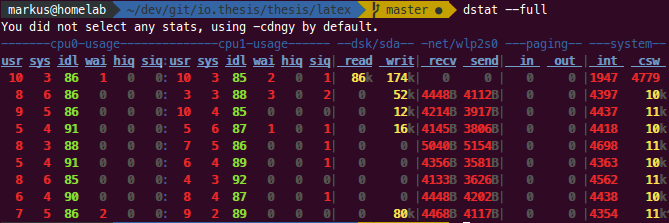
\includegraphics[width=1.0\textwidth]{../images/06-dstat-full.png}
	\caption{Output "dstat --full"}
	\label{dstat-output}
\end{figure}

Additionally, Dstat provides multiple parameters to specify the data to be displayed, e.g.
--cpu, --disk, --net, and many more. Used in combination, the data can be grouped in the
following categories according to the parameters:

\begin{table}[H]
    \begin{tabular}{ll}
        \textbf{Category} & \textbf{Dstat parameters} \\
        cpu & ("--cpu", "--top-cpu-adv", "--top-cputime", "--top-cputime-avg")\\
        disk & ("--disk", "--disk-tps", "--disk-util")\\
        net & ("--net", "--socket", "--tcp", "--udp")\\
        io & ("--io", "--top-io-adv", "--lock", "--fs")\\
        memory & ("--mem", "--top-mem", "--page", "--swap", "--vm")\\
        system & ("--sys", "--load", "--ipc", "--unix")\\
        process & ("--proc", "--proc-count", "--top-latency", "--top-latency-avg")\\
    \end{tabular}
    \caption{Dstat data categories}
    \label{tbl:dstatcategories}
\end{table}

Although the parameters are mostly self-explanatory, a list containing short descriptions
for each of the parameter used in Chapter 4 Architecture and Implementation is available in
Appendix. TODO Based on the data in the extracted categories, Dstat can be considered
as a source that gives a fairly complete picture of the state of a system.

Dstat is a tool only available for unix systems, and therefore not available for Windows or
Macintosh. Since Apache Flink and Apache Kafka are operated on Unix systems in most
cases, this fact can be neglected because this tool offers a wide range of data to describe
the system state a certain point of time.

\subsection{Application data}

Every application running on the Java Virtual Machine, can be accessed via JMX as discussed
in Chapter 2 Basic Concepts. According the specification, every implementation of the JVM contains
implementations for a basic set of management interfaces, that enables the access separate parts of JVM related data,
located in the package "java.lang.management" \cite{Javadoc16}.

\begin{table}[H]
    \begin{tabular}{ll}
        \textbf{Management interface} & \textbf{JMX ObjectName} \\
        ClassLoadingMXBean & java.lang:type=ClassLoading \\
        OperatingSystemMXBean & java.lang:type=OperatingSystem \\
        RuntimeMXBean & java.lang:type=Runtime \\
        ThreadMXBean & java.lang:type=Threading \\
        MemoryMXBean & java.lang:type=Memory \\
        BufferPoolMXBean & java.nio:type=BufferPool,name=* \\
        GarbageCollectorMXBean & java.lang:type=GarbageCollector,name=* \\
        MemoryManagerMXBean & java.lang:type=MemoryManager,name=* \\
        MemoryPoolMXBean & java.lang:type=MemoryPool,name=* \\
    \end{tabular}
    \caption{"Default" JMX JVM data}
    \label{tbl:jmxjvmdata}
\end{table}

There's a difference in the way of data access between the object name containing an asterisk "*"
and the one the ones that doesn't. The asterisk indicates the existence of multiple MBeans for a given query string,
the result of a query for the object name "java.lang:type=GarbageCollector,name=*" results in multiple data sets according
to existing garbage collector names.

This "default" set of management interfaces provides a deep insight into JVM data, is
available for Apache Flink and Apache Kafka and will be included in the software solution
in Chapter 4.

\subsubsection{Apache Flink}

Apache Flink provides application data via its monitoring API, a RESTful API, see
Chapter 2 Basic Concepts, that delivers JSON data based on HTTP
GET requests. It can be used to query general cluster information and status and
statistics of running and completed jobs. The dashboard that comes with Apache Flink
uses this monitoring API, but is designed to be used also by custom monitoring tools. The
monitoring API runs as part of the JobManager and listens at post 8081 by default. All requests
are of the sample form http://hostname:8081/jobs, below a list of available REST resources that
will be used to fetch cluster- and job-related data for Apache Flink in Chapter 6 Implementation,
see Appendix A for the corresponding JSON responses.

\begin{table}[H]
    \begin{tabular}{ll}
        \textbf{API path} & \textbf{Description} \\
        /config & Server setup \\
        /overview & Cluster status \\
        /jobs & Job ids by status running, finished, failed, canceled. \\
        /jobs/{jobId} & Job details, dataflow plan, status, timestamps of state transitions \\
        /jobs/{jobId}/exceptions &  Exceptions that have been observed by the job \\
        /jobs/{jobId}/config & User-defined execution config used by the job \\
    \end{tabular}
    \caption{HTTP monitoring endpoints Apache Flink}
    \label{tbl:http-api-flink}
\end{table}

Appendix A provides a list with sample JSON response according to this REST endpoints. TODO

Since version 1.1.0, Apache Flink also provides a rudimentary metrics system that exposes
basic data for the Java Virtual Machine, the JobManagers and TaskManagers are running
on. This data includes inter alia cpu usage or memory consumption, as well as basic
information about running jobs. According to the "default" JVM data described in Table 3.2
and the data provided by the monitoring REST api, the metrics system in its current version
represents just an excerpt of the data that will be collected anyway.

\subsubsection{Apache Kafka}

In addition to the standard interfaces and MBeans that come with the implementation
of the JVM, Apache Kafka provides a set of managed resources providing application
specific metrics concerning the Kafka domain, reaching from global broker metrics, global
connection metrics to metrics per topic like in- and outgoing byte rates for example. Based
on the requirement to collect as much data as possible, the data of all provided resources
will be collected, the complete list of MBeans observed for Apache Kafka is available in
Appendix A.

\subsection{Data Quality}

The following introduces to the basics of the term "Data Quality" for inspection the data sources
described above based on common quality criteria.

Data quality refers to the quality of data as it is provided by measurements and describes the
ability of data to represent the mapping from an empirical system("the real world" we operate in)
to the numeric system correctly with the main goal to satisfy a given need or objective.
It can not be expressed quantitatively, but \cite{Daqua13} and  \cite{Ebert07} introduce multiple
common criteria for measuring the quality of data, from which a selection is made to check the data
previously described on their quality:

\begin{enumerate}
    \item \textbf{Correctness:}
    The data correspond to the entities of the real world, that is, the data represent the reality.

    \item \textbf{Consistency:}
    Recorded data sets does not show discrepancies, logical contradictions or errors when compared
    among themselves.

    \item \textbf{Reliability:}
    The origin of the data is traceable and the sources are trusted.

    \item \textbf{Completeness:}
    The required information is available and no data values are missing or in an unusable state.

    \item \textbf{Accuracy:}
    Expresses the mapping from the empirical system to the intended numerical system. Recorded values
    conform to actual values,

    \item \textbf{Timeliness:}
    All data records correspond to the current state of the modeled world and thus are not outdated.
    The data are the actual properties of an object from a timely manner.

    \item \textbf{Redundancy-free:}
    The data does not contain any duplicates, where a duplicate is meant to be data describing the same entity
    in the real world.
\end{enumerate}

\subsection{Results}

According to the examinations of system and application data available for Apache Flink and Apache Kafka,
the following matrix of data sources results for both of the systems:

\begin{table}[H]
\begin{tabular}{lll}
 & \textbf{Apache Flink} & \textbf{Apache Kafka} \\
\textbf{System data (Dstat)} & X & X \\
\textbf{JVM data (JMX)} & X & X \\
\textbf{Application data (JMX)} & X & X \\
\textbf{Application data (REST)} & X & - \\
\end{tabular}
\caption{Data source matrix}
\label{data-source-matrix}
\end{table}

Regarding the criteria of Data Quality, the following statements can be made:

\begin{enumerate}
    \item The extracted data sources provide snapshot of system and application related data at a
    given point of time and thus are not outdated. They meet the criterion \textbf{Correctness}.
    \item The data sources are well known and trusted, therefore they are \textbf{reliable}.
    \item The Consistency of data needs to be evaluated be comparing data sets over a period of time,
    but will be assumed because the data sources are based on known applications and specifications.
    \item The data is \textbf{accurate}, they represent the "real world" with a description of the state of the
    underlying system.
    \item The data is \textbf{timely}. Dstat, JMX and REST data describe the state at the point when the data is
    queried.
    \item The data is not redundancy-free! The "default" JMX data provided by the implementation of the JVM and the
    application data for Apache Flink available since version 1.1.0 both contain cpu, memory, garbage-collector, et al,
    data based on the management interfaces listed in Table 3.2. The same applies for the data available via Apache Flink's
    monitoring API and the application metrics regarding jobs and Job-/TaskManager information.
\end{enumerate}

To summarise the results of the data analysis, there're three different sources for collecting system and application
data for Apache Flink and Apache Kafka. The Dstat system tool for unix-based system provides technical data on the
lowest level of abstraction. On a higher level, application data is provided by JMX for both of the systems containing
application-related data, like broker metrics for Apache Kafka or job information for Apache Flink, but also "default"
JVM data for all Java based systems. The JMX metrics system of Apache Flink exists since version 1.1.0 (Release date
9th of August 2016) and represents a current feature, which is not fully developed yet according to the JIRA of
Apache Flink. The full set of Flink related application data is exposed via its HTTP
monitoring API.

According to the criteria introduced above, a certain level of Data Quality can be assumed, because the data sufficiently
matches these criteria except. The only exception is the criterion that requires data to be free of redundancies. The metrics
for Apache Flink are just a very small excerpt of the JVM and application related data that will be collected anyway according
to Table 3.2 and Table 3.3.

\section{Functional Requirements}

The main goal of the thesis is a working software system to collect system and application data available
for Apache Flink and Apache Kafka. Furhermore, the collected data must be stored in a
persistence system to become available for possible consumers like visualization applications,
analytical processes or as a data source for applications from the context of Machine Learning
for example.

From this, three main functional requirements derive:
\begin{enumerate}
    \item Collection of data from Apache Flink and Apache Kafka source systems.
    \item Storage of collected data in a persistent medium.
\end{enumerate}

In preparation of this thesis my supervisor Prof. Dr. Stefan Edlich once said \textit{"Sie sammeln
alles, was nicht bei drei auf dem Baum ist"}, which leads to the requirement to collect as much data
as possible. As a result, available data sources for has been inspected in the previous secion and the
software solution must provide a mechanism to collect data from the sources discussed in the data source
matrix shown in Table 3.4.

The collected data must be brought into format, that enables transmitting and storing structured data.
Because nowadays usually the JavaScript Object Notation (JSON) is used for transmitting and storing
structured data, the data collected on Apache Flink and Apache Kafka must be transformed into its JSON
representation, before the data will be transmitted to the storage system. Another advantage of JSON is
that it independent of any programming language, parsers for any language are available.

At the time of this thesis, the concrete usage scenarios of the collected data are not yet known.
As is not yet known when the data is needed, the process of data collection must provide a mechanism
to collect the data "on demand" and therefore an interface to start and to stop the collection process.
This results in the advantage that the data is collected only when necessary to minimize the consumption
of resources on the source systems as well as the memory consumption in the storage system.

In addition to the collection on source systems, data must be must be stored on a centralized storage system
to become available for potential data consumers, which are unknown at present. The data must be held in a
common format to be accessible to a variety of consumers. Since JSON is a standard format for exchanging data,
the collected data will be in JSON format, therefore the storage system must be able to store and to query
JSON data.

This results in the following functional requirements:

\begin{itemize}
	\item Collect Dstat system utility data for both systems
	\item Collect "default" JVM data using JMX for both systems
	\item Collect application data using JMX for both systems
	\item Collect application data using REST for Apache Flink
	\item Data must be transfered into a JSON model
	\item Data must be stored in JSON format
\end{itemize}

\section{Non-Functional Requirements}

In addition to the functional-requirements that describe what the software solution is supposed
to accomplish, the next section introduces the non-functional requirements, sometimes refered to as
"quality attributes" of a system, that essentially specify how the system should behave and represent
constraints upon the systems behaviour.

\begin{enumerate}
    \item \textbf{Performance:} the data collection implementation doesn't cause a negative impact regarding
    system resources like cpu or disk usage on the systems. On architectural level, the collected data should be
    available in the database in real-time / near real-time. A duration of 2 seconds from leaving the source system until
    it arrives in the storage system is set as a criterion.

    \item \textbf{Extensibility:} The collector architecture should be easy to adapt for other source systems
    like Apache Spark,independent of programming languages used for the collection and storage of data.

    \item \textbf{Scalability:} Apache Flink and Apache Kafka systems are composed of several interacting components, they
    operate in clustered environments. The software must be scallable in a way, where it does not matter whether to collect
    data from a single system or multiple nodes in a cluster. Similarly, the consumers of the data are still unknown. Therefore
    there is a requirement that consumers can be integrated in the infrastructure easily.
    Furthermore, it has be ensured at the level of implementation that the software solution scales for further data sources,
    that might arise in the future, like additional resources in Apache Flink's monitoring API.

    \item \textbf{Portability:} The solution must not be dependent on which storage technology is used. A change of the
    database may not affect the data collection process.

    \item \textbf{Simplicity:} Data consumers and producers should be independent in the way that no specialized operations
    for interchanging data are required.

\end{enumerate}

\section{Summary}